\documentclass[11pt,leqno]{article}

\usepackage{amssymb}
\usepackage{amsmath}
\usepackage{mathrsfs}
\usepackage{xcolor}
\usepackage{mathrsfs}
\usepackage{hyperref}
\usepackage{comment}
\usepackage{graphicx}
\usepackage{indentfirst}
\graphicspath{ {./} }

\textwidth              16 cm
\textheight             24.5  cm
\oddsidemargin          -1   cm
\evensidemargin         -1cm
\topmargin              -1 cm
\setlength{\evensidemargin}{15.5pt}
\setlength{\oddsidemargin}{2.5pt}

\pagestyle{empty}

\def\ClasaO{{\mathcal O}}

\usepackage{algpseudocode}

\title{Tema 2}
\author{Mihai Cristian-Laurentiu 2B4, Stamate Valentin 2B4}
\date{23.11.2020}

\begin{document}

\maketitle

% 

\section*{Problema 1} 
a. Cosideram pentru urmatoarea demonstratie relatia $|S|\leq |T|$ deoarece cuplajul satisface intotdeauna clasa cu cardinalul cel mai mic din bipartitie.\\
Presupunem ca exista un cuplaj M care satureaza toate nodurile din S, si demonstram  ca se satisface conditia lui Hall $\forall A\subseteq S$.
Fie M(A) multimea tuturor varfurilor din T satisfacute de cuplajul M, pt o multime A fixata. Din definitia cuplajului $|M(A)|=|A|$, dar $M(A)\subseteq N_G(A)$ deoarece toate varfurile din M(A) sunt vecini cu varfurile din A. Astfel $|N_G(A)|\geq|M(A)|$, deci $N_G(A)\geq |A|$. Deci exista un cuplaj care satisface o clasa a bipartitiei\\

b. In continuare vom incerca sa explicam o strategie pentru aflarea celei de-a sasea carte. Fie ce doi prieteni, 
Dealerul ( cel care va face trucul), si Jucatorul( cel care va "ghici" cartea).Vom folosi doar 5 din cele 6 carti, astfel ce-a de cincea carte 
plasata nu va fi necesara pentru aflarea celei ascunse. Dealerul alege cartile pe care le va arata, cat si ordinea lor. Exista $\mathcal C_5^4$ 
modalitati de a alege 4 din 5 carti si 4! moduri de a ordona cele 4 carti (primele patru). Jucatorul poate decoda realtiv usor 24 de combinatii 
dar mai greu cele 120. O metoda pentru a decoda mai usor mai mult de 24 de combinatii este sa observe,folosind principiul lui Dirichlet, ca in cele 
5 carti pe care Dealerul le foloseste trebuie sa exista cel putin doua de acelasi semn. Prima carte pe care Dealerul o va arata este una din acea 
pereche de doua, iar a doua (pe care nu o va arata) este cartea care urmeaza a fi ghicita. Presupunem ca ordonam cartile crescator de la A,2,3,..,K si 
le plasam intr-o ordine circulara (astfel dupa K urmeaza 1,2,...) si definim distanta intre cartea a si cartea b, distanta(a,b) ca fiind distanta pe 
cerc de la a la b. Astfel pt orice doua carti a,b $|distanta(a,b)|\leq 6$. Daca distanta ar fi 7 sau mai mare atunci ar trebuie sa existe cel putin 14
 carti in cerc. De exemplu, fie cartile 4 si Dama (D), Dealerul va arata ca prima carte Dama pentru ca distanta(D,4)= 5. Apoi Dealerul alege o ordonare
  a celorlalte 3 carti (a patra nefiind necesara) pentru a codifica un numar de la 1 la 6. Jucatorul decodifica acest numar si il aduna primei carti 
  pentru a afla cartea ascunsa. Exista multe moduri de a identifica un numar de la din permutarea celor 3 carti. Vom folosi in ordine de la 1 la 6: (123), (213), (231), (132), (312), (321). 
  Pentru a afla permutarea, pozitia celei mai mici carti ne spune 1,2,3 . Din ordinea celorlalte doua vom sti daca sa adaugam sau nu 3; 
  daca sunt in ordine crescatoare (2,3) vom adauga 3, in caz contrat nu. Pentru a putea face ordonarea corecta vom presupune ca daca doua 
  carti au aceeasi valoare se vor ordona dupa simbolul carti, ordinea fiind fixata de cei doi prieteni in prealabil (Frunza, Inima, Trefla, Romb: $ \clubsuit, \diamondsuit, \heartsuit,\spadesuit$.

Exemplu: Presupunem ca Dealerul are cartile $3 \diamondsuit , 6 \diamondsuit,8 \spadesuit,10 \clubsuit$ si $8 \heartsuit$, si oricare alta ( care nu este necesara pentru a afla cartea ascunsa, o vom nota C ). 
Deaorece avem doua carti de Romb, Dealerul va ascunde $ 6 \diamondsuit$ sau $3 \diamondsuit$. 
Dealerul ascunde $6 \diamondsuit$ ( sau cealalta de romb, nu este important,distanta dintre cele doua este 3) si afiseaza secventa $ 3 \diamondsuit,8 \spadesuit,10 \clubsuit,8 \heartsuit, C$ care codifica 3. 
Permutarea este (231), 2,3 fiind in ordine nu vom adauga 3, ca in cazul (321). Din punctul de vedere al Jucatorului, vazand secventa , 
vede simbolul cartii ascunse (din prima carte) si combanatia urmatoarelor 3 care codifica numarul 3, adauga 3 primei carti si afla raspunsul corect ($6 \diamondsuit$), 
acesta fiind numarul primei carti si simbolul acestei + numarul dat de permutare.

%

\section*{Problema 2}
    a. Stim din definitia din curs: $G$ este n-conex daca $ G / A $ este conex $ \forall A \subseteq V(G) \; |A| < n $.
Cum $ A = \{x\} | x \; server $ ,atunci trebuie sa demostram ca G este 2-conex. 
Din enuntul problemei stim ca doi clienti nu pot fi conectati unul cu altul si ca nu pot comunica decat cu serverele deoarece clientii nu pot ruta mesaje.
Astfel, un client poate comunica cu un server doar daca serverele se afla se afla intr-o componenta conexa. In cazul minimal subgraful indus de multimea serverelor va fi arbore.
Atunci adaugand muchiile dupa cum ne spune proprietatea, vom obtine un graf $G'$ care este 2-conex. 

    Demostratie: Presupunem prin reducere la absurd ca subgraful indus de multimea serverelor ($G'$) se deconecteaza la eliminarea unui nod x. Insa vecinii lui x din cele doua componente conexe vor fi conectati printr-o muchie deoarece se aflau la distanta 2, astfel vom obtine o contadictie. 
    
    Cum fiecare nod din $G'$ are gradul cel putin 2 atunci la eliminarea unui server toti clientii vor avea gradul cel putin 1 insemnand ca fiecare client va ramane conectat cu cel putin un server si ca poate comunica cu toate celelalte servere,
    graful $G'$ fiind 2 conex astfel daca un server cade, reteaua va ramane conexa.

    b. Fie $G$ graful asociat retelei, $G'$(graful dupa modificare), $H$ si $H'$ subgrafuri induse de multimea serverelor in $G$ respectiv $G'$. Ponind tot de la un caz minimal unde $H$ este un arbore, putem observa urmatorul lucru.
Modul cum adaugam muchiile este similar cu modificarile aduse la subpunctul a doar ca nu mai avem restrictia de a trasa o muchie la distanta 2. Astfel noi trebuie sa adaugam doua muchii pentru fiecare doua noduri conectate direct. Aceste muchii se vor crea doua cicluri de lungime minim 2 iar aceste cicluri se vor intersecta in muchia dintre cele doua servere.
Astfel fiecare nod avand un vecin dupa modificare vom obtine subgraful $H'$ in care fiecare nod va avea gradul cel putin 3 deoarece pentru un nod oarecare cu grad cel putin 1 va trebui sa adaugam alte doua muchii pentru obtinerea a doua circuite. La fel si pentru nodurile care au deja grad cel putin 2: va trebui sa adaugam o muchie pentru a obtine doua circuite. Daca in graful minimal $H$ ar fi fost mai multe muchii proprietatea nu s-ar fi schimbat deoarece muchiile suplimentare ar fi facut parte din circuitele adaugate anterior.
Astfel cum fiecare nod din $H'$ are gradul cel putin 3 putem spune ca este 3-muchie-conex deoarece daca am sterge doua muchii am avea unele noduri cu grad cel putin 1 si s-ar pastra conexitatea in $H'$. Atunci reteaua ramane conectata daca ar cadea doua conexiuni directe dintre servere. Q.E.D. 

\section*{Problema 3} 
a.
"$\Rightarrow$" 
Fie $H_1$, $H_2$ doua b-subgrafuri, iar H un subgraf astfel incat $H = (H_1 \cap H_2)$. H contine strict pe $H_1$ (sau $H_2$) deci din proprietatea din enunt acesta nu mai este 2-conex, astfel prin eliminarea nodului in care $H_1$ intersecteaza $H_2$ subgraful H se deconecteaza, deci nodul de intersectie este punct de articulatie.\\

"$\Leftarrow$"
Fie x punct de articulatie in G. Stim ca $G \setminus {x} = G'$ are doua componente conexe $H_1$ si $H_2$ iar $|V(b-subgraf)| \geq 2$.
Astfel $H_1 \cup {x}$ este conex dar si $H_2 \cup {x}$ este conex. Deoarece un b-subgraf are minim doua noduri, pornind de la x putem construi un
b-subgraf = $B_1$ in $H_1$($B_1\in G$) care nu are noduri in $H_2$(exceptie nodul comun) deoarece adaugand un nod din $H_2$ vecin cu x, el se va deconecta la stergerea acestuia iar proprietatea de
b-subgraf nu mai este indeplinita. 

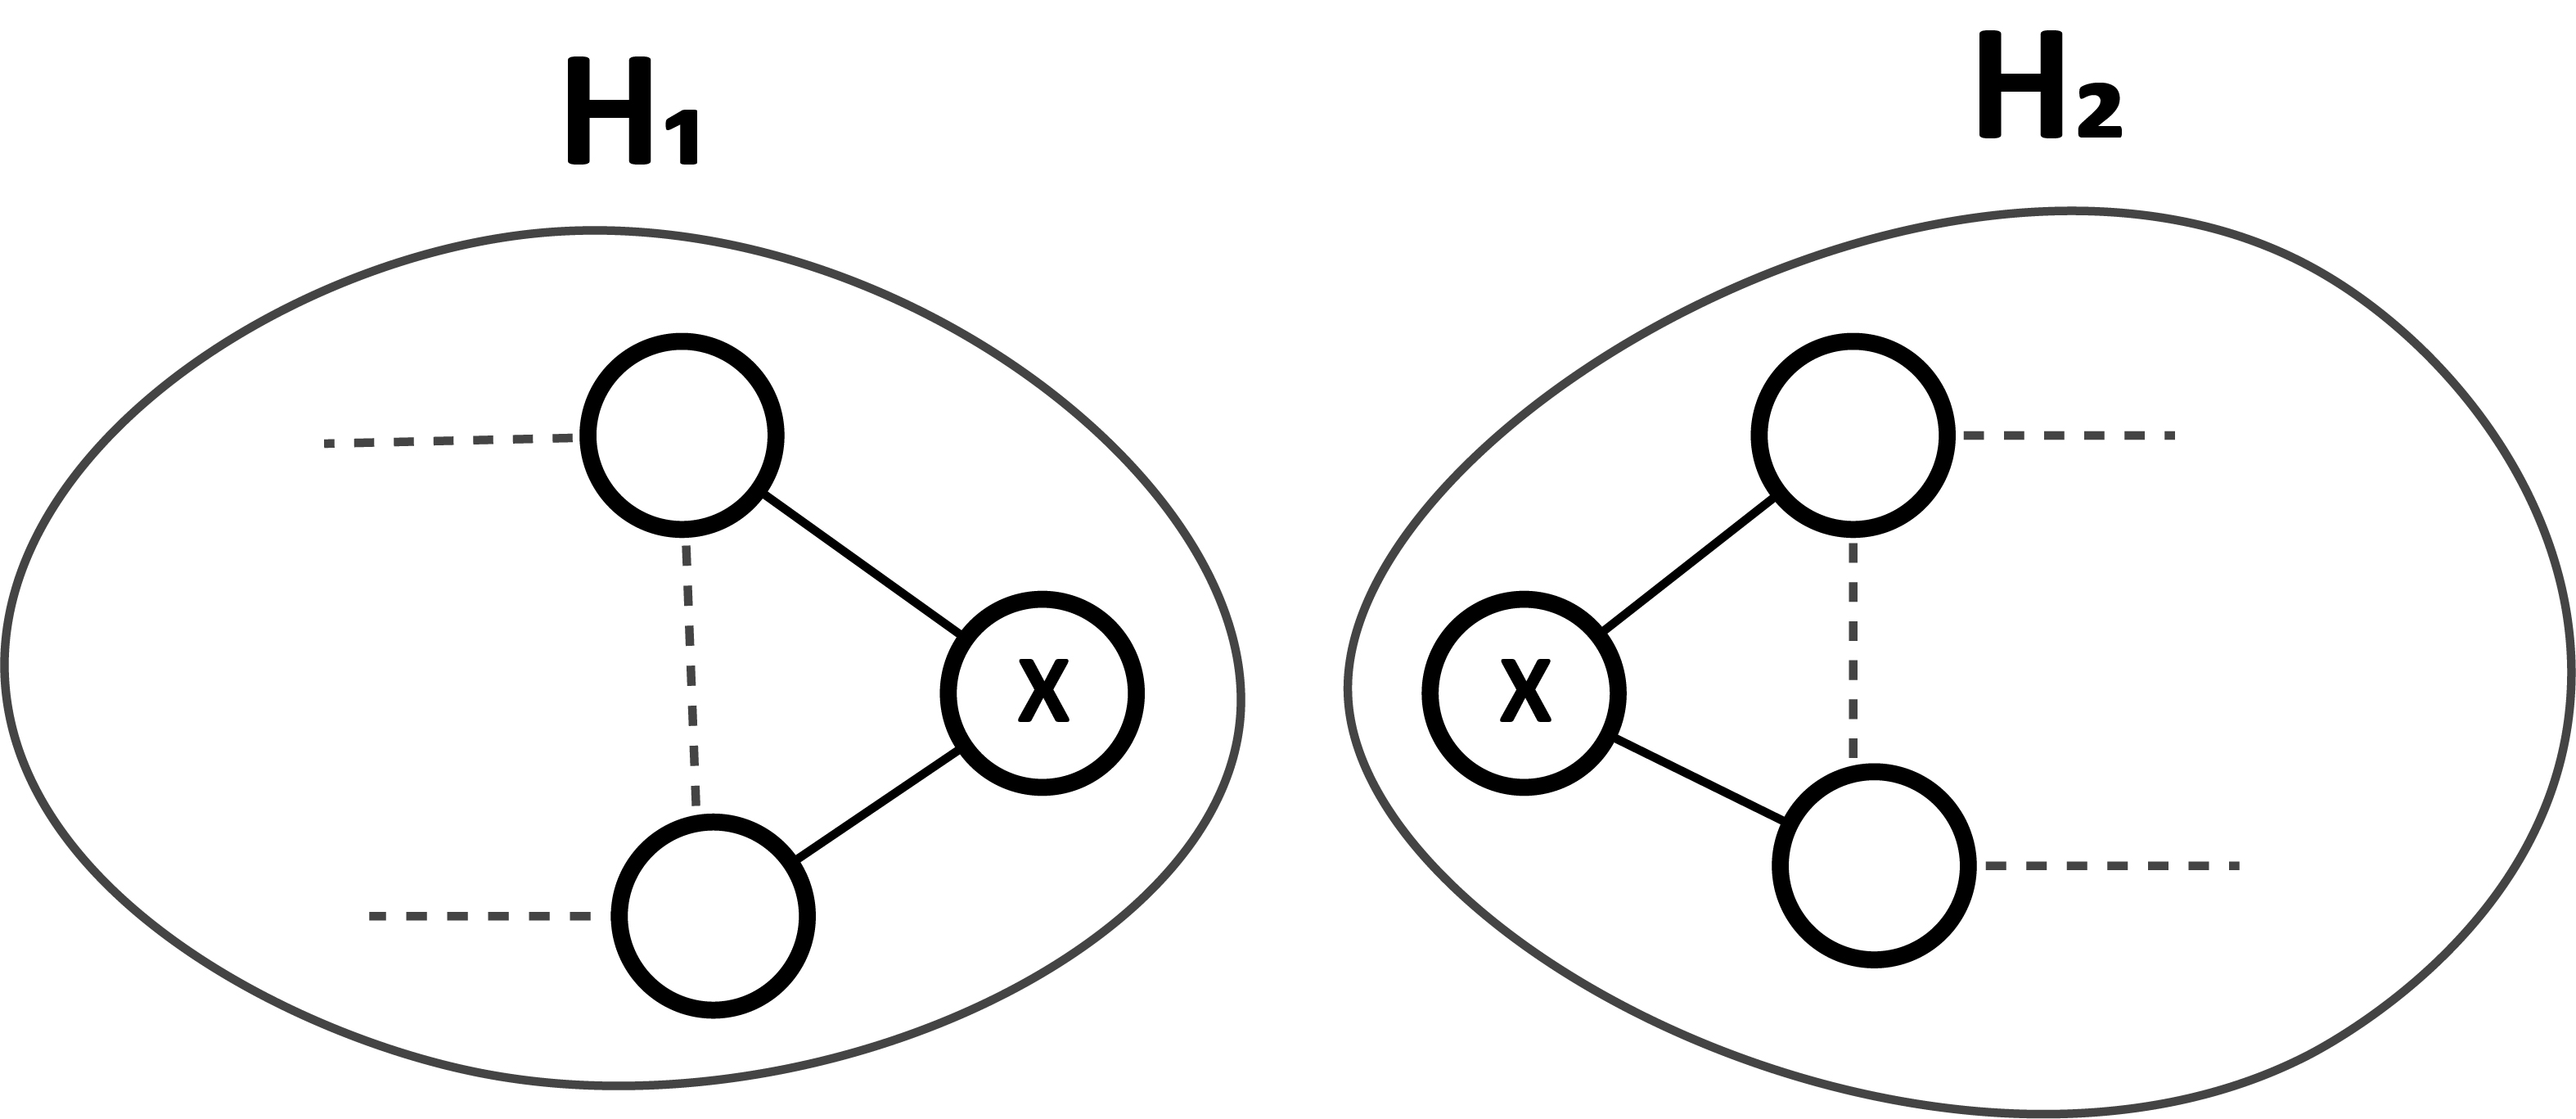
\includegraphics[width=\textwidth]{grap_ex3_2.jpg}

In mod analog si pentru $H_2$. Astfel demonstrand ca un punct de articulatie x din G, se afla la intersectia a doua b-subgrafuri.

Facand cele doua demostratii putem trage concluzia ca un punct de articulatie se afla la intersectia a cel putin doua b-subgrafuri si intersectia a cel putin doua b-subgrafuri 
este un punct de articulatie. Q.E.D. 

b. Stim de la subpunctul a ca orice punct de articulatie in $G$ se afla la intersectia a cel putin 2 b-subgrafuri. 
Astfel multimea nodurilor care se afla la intersectia a cel putin doua b-subgrafuri din G este
chiar multimea $\mathcal{V}_2$.

    i. $\mathcal{G}$ conex: Multimea $\mathcal{V}_2$ este formata din intersectia nodurilor ce se afla la intersectia b-subgrafurilor din $\mathcal{V}_1$(subpunctul a). 
    Cum graful G este conex, atunci stim ca exista un drum intre doua noduri care sunt puncte de articulatie(adica din multimea $\mathcal{V}_2)$
    Daca $\mathcal{G}$ nu ar fi conex atunci nu va exista un drum de la doua noduri oarecare din $\mathcal{V}_2$. 
    Acest lucru inseamna ca nici G nu ar fi conex deoarece fiecare nod $x \in \mathcal{V}_2$ 
    este conectat cu cel putin doua b-subgrafuri din $\mathcal{V}_1$. Ceea ce este contradictie cu proprietatea de conexitate a lui G.
    Astfel $\mathcal{G}$ este conex.

    ii.$\mathcal{G}$ aciclic: Cunoscand faptul ca un b-subgraf este maximal, existenta unui ciclu in $\mathcal{G}$ ar determina existenta unui alt b-subgraf 
    ce nu apartine lui $\mathcal{V}_1$ deoarece un ciclu formeaza un b-subgraf. 
    Asta ar insemna ca proprietatea de b-subgraf nu este maximala ceea ce este contradictie. Astfel am demostrat ca $\mathcal{G}$ este aciclic.

    Facand cele doua demonstratii i si ii rezulta ca $\mathcal{G}$ este un graf conex si aciclic adica un arbore. Q.E.D
 
c. Algoritmul este bazat pe o parcurgere DFS iar nodurile sunt vizitate recursiv de la nodul de start
in ordinea data de nodurile nevizitate nodului curent. 

Cum tabloul order[] nu se modifica decat la inceputul fiecarui
apel recursiv, el va retine ordinea de vizitare DFS al oricarul nod.

Pentru tabloul high[] observam ca pentru un vecin care a fost deja vizitat ii schimbam valoarea cu $min(high[x], order[v])$
iar la intoarcerea din recursie schimbam valoare lui high[x] in $min(high[x], high[v])$
Putem observa ca pentru un nod al carui high[x] a fost schimbat, valoare lui se va propaga printre toti parintii
pana vom ajunge la nodul care corespunde cu vecinul nodului de la care a inceput shimbarea lui high[x].
In acest moment stim sigur ca $order[x] \leq high[x]$ iar nodul x va fi afisat ca si punct de articulatie.
Mai observam ca atunci cand un nod are ca vecin un nod deja vizitat($order[x] != -1)$ atunci putem deduce
ca exista un ciclu intre cele doua noduri(cazul minimal al unui b-subgraf). 
Astfel, algoritmul marcheaza nodurile cu o valoare $k_i$ care formeaza un circuit dar si acele noduri din circuit care formeaza alte circuite.
Prin aceasta marcare recursiva vom ajunge la un b-subgraf deoarece eliminand un nod dintr-un circuit el va ramane conex. Un exemplu este dat in imaginea urmatoare:

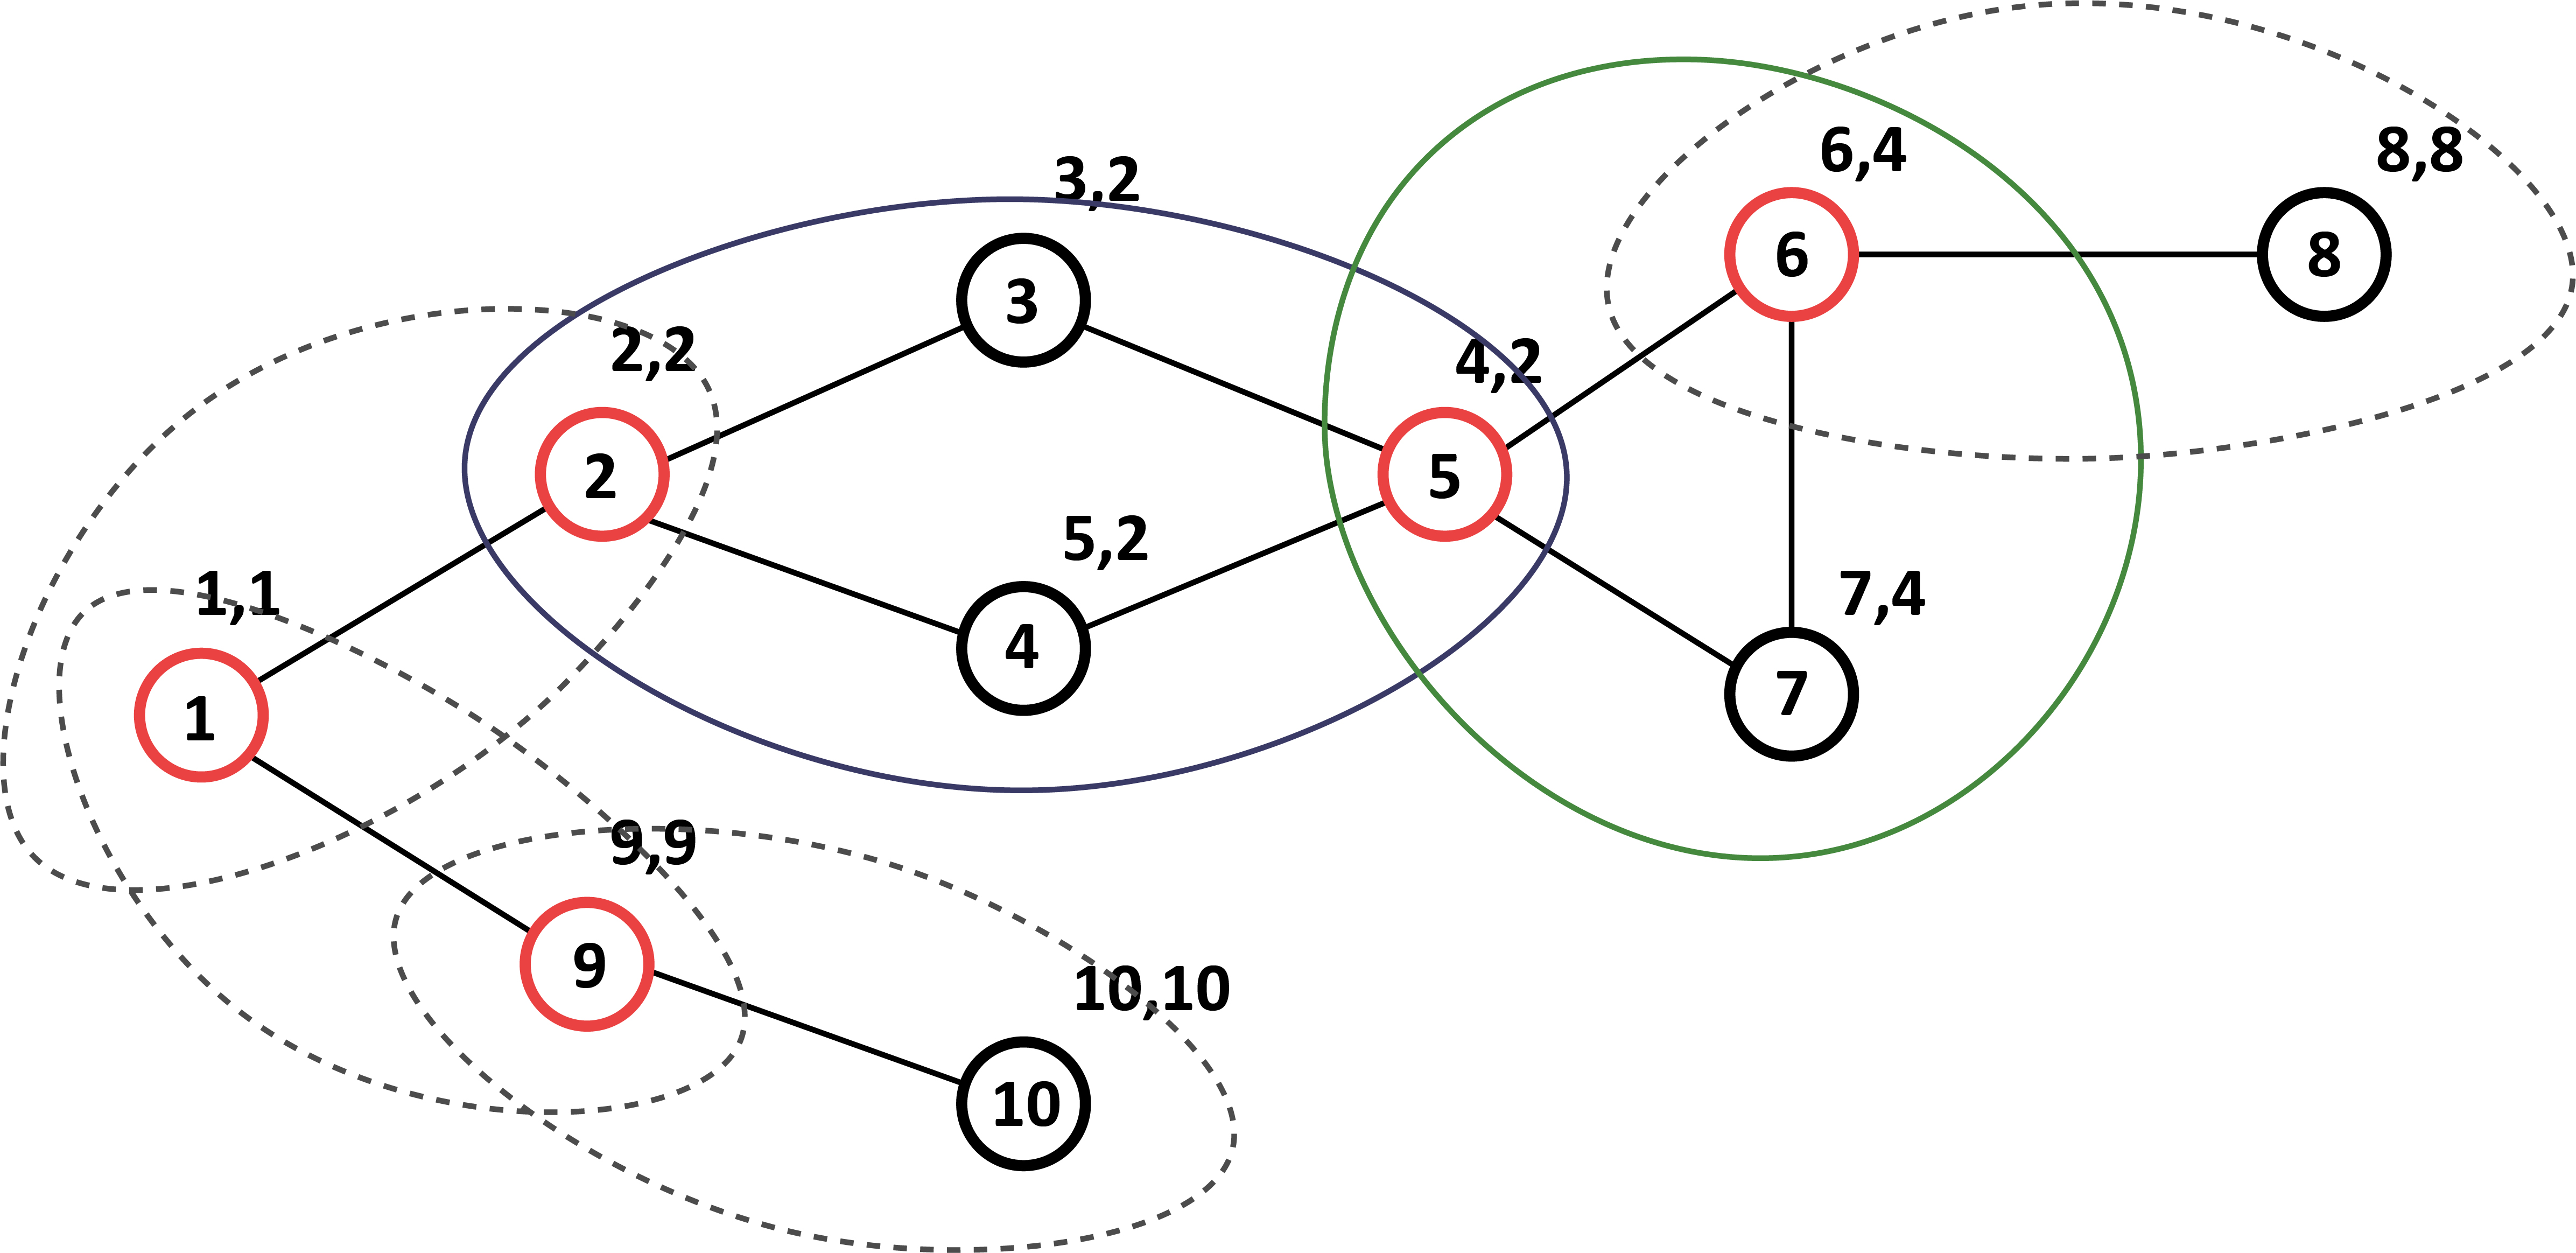
\includegraphics[width=\textwidth]{grap_ex3_1.jpg}

 - x, y corespunde cu valoare lui order respectiv high

 - liniile continue sunt b-subgrafuirle in care valoare lui high este eceeasi cu exceptie in unele cazurile in care doua b-subgrafuri se intersecteaza

 - liniile punctate corespund cu b-subgrafuri pe care algoritmul nu le "marcheaza" in mod direct, ele respectand celelate conditii explicate mai jos

 - nodurile cu rosu sunt afisate de algoritm ca si puncte de articulatie.\\

    b-subgrafurile de oridin 2 nu sunt marcate direct dar pentru un nod c care are cel putin doi vecini
    se si e punct de articulatie se va respecta conditia $order[x] \leq high[v]$(x si v sunt adiacente formand un b-subgraf).
    Astfel fiecare nod ce se afla la intersectia a doua b-subgrafuri va fi afisat ca si punct de articulatie.
    Este usor de vazut pentru nodul radacina(primul nod vizitat) ce are cel putin doi copii si nu exista un circuit dat de cele 3 noduri(radacina si cei doi copii), el va fi punct de articulatie si va fi afisat corect de algorithm.
    Astfel algoritmul de mai sus este corect: el afiseaza toate punctele de articulatie.


% 

\section*{Problema 4} 

Demostratie ajutatoare pentru b si c: Demonstram prin inductie ca dupa terminarea fiecarei bucle for T va fi format din arbori partiali de cost minim.

Verificare: pentru p = 2 avem 2 noduri care vor fi conectate cu singura muchie din graf. Dupa terminarea buclei for T va fi compus dintr-un singur arbore partial de cost minim: graful initial.

Presupunem ca T neconex si $ T = \{T_{1}, T_{2}, ..., T_{p}\} $, unde $ T_i, i = 1, p $ este arbore partial de cost minim in subgraful indus de $V(T_i)$ in $G$ si demostram ca dupa terminarea buclei for $T = \{T_{1'}, T_{2'}, ..., T_{p'}\}$ unde $T_i, i = 1, p'$ este arbore partial de cost minim in subgraful indus de $V(T_i)$ in G.
Fie $e$ muchia de cost minim cu capetele in doi arbori partiali de cost minim din T: $ T_i$ respectiv $T_j$ $ i != j$, $i = 1,p$ $j = 1,p$.
Unind cei doi arbori vom obtine un arbore $T_k$ si este de cost minim in subgraful indus de $V(T_k)$ in $G$ deoarece muchia adaugata are costul minim in G si uneste alti 2 arbori partiali de cost minim. Acest arbore este unic deoarece toate muchiile au costuri diferite.
$T$ se va modifica astfel $T = T \setminus \{T_i, Tj\} \cup T_k \ $, iar proprietatea lui T de a avea ca si componente arbori partiali de cost minim este pastrata. Repetand procesul, vom iesi din bucla for iar
$T = \{T_{1'}, T_{2'}, ..., T_{p'}\}$ unde $T_i, i = 1, p'$ arbore partial de cost minim, ceea ce trebuia demonstrat.


a. Adaugand cate o muchie e ($ e=uv$ : $uv \in E, u \in V(T_i), v \notin V(T_i)$) care conecteaza doua componente conexe deiferite se obtine o noua componenta conexa. 
In cazul cel mai nefavorabil se conecteaza doua componente care nu au fost conectate la pasii precedenti din bucla for, astfel numarul de componente conexe rezultat dupa executia buclei for va fi jumatate ( mai exact $\lceil p/2 \rceil$, unde p este numarul de componente conexe inainte de executia buclei for).

b. Initial exista p=n componente conexe (varfurile din graful G), acestea fiind aciclice. Deoarece o muchie uv conecteaza doar componente conexe diferite ($u \in V(T_i), v \notin V(T_i)$), oricare doua componente vor fi conectate prin exact o muchie,
astfel noile componente conexe rezultate vor fi aciclice. Stim acest lucru din demostratia ajutatoare de mai sus. 
In concluzie, la terminarea executiei buclei while, T va fi conex iar fiind format din componenete conexe aciclice conectate prin exact o muchie, va fi la  randul lui aciclic.


c. La fiecare pas din bucla for se alege muchia de cost minim care conecteaza doua componente conexe diferite (arbori partiali de cost minim, cunoscand acest lucru din demostratia de mai sus). 
Astfel alegand la fiecare pas muchia de cost minim, graful rezultat fiind aciclic si functia de cost fiind injectiva T rezulta un arbore partial de cost minim.

d. Din a.$\Rightarrow$ ca dupa fiecare iteratie while numarul de componente conexe se injumatateste (cel putin). Bucla se opreste cand se obtine un graf conex deci numarul de iteratii while este $\ClasaO(log_2 n) \subset \ClasaO(log n)$.\\
La fiecare iteriatie while algoritmul cauta muchia de cost minim astfel in cel mai nefavorabil caz se va parcurge (in bucla for) toata multimea de muchii E ($|E|=m$), astfel complexitatea fiecarei iteratie while este $\ClasaO(m)$.\\
In concluzie complexitatea finala a algoritmului este $\ClasaO(m\;log n)$.


\end{document}
